\renewcommand{\chaptername}{\scshape Partie}
\chapter{\normalfont \scshape Photographie de l'onde de choc}
\section{Résultats attendus et limites}
D’après la relation \ref{indice_pression} (c.f. Partie 1), un autre moyen de faire varier la masse volumique du milieu est de changer la pression: c’est ce que fait une onde de choc. On fait l’hypothèse que la pression au niveau de l’onde de choc observée est la même que la pression à la rupture de la membrane (\textbf{$P$ = 2,5 bar}), ainsi, en utilisant à nouveau la relation des gaz parfaits, on en déduit une variation d’indice optique très forte  : \\
\centerline{$\frac{\Delta n}{n}$ = \textbf{39,7 \%}}\\ \\
On s'attend donc à ce que le contraste soit bien visible dans l'image de l'onde de choc. Cependant, vu la grande variation de pression, l'onde de choc se propage à très grande vitesse. En effet, d'après la loi de \textsc{Mach} :
\begin{align}
	c= \sqrt{\gamma\,\frac{P}{\rho}}
\end{align}
Or, $\gamma = \frac{7}{5}$, ce qui donne à peu près \textbf{$c$ = 520 m/s} à \textbf{2,5 bar}.\\\\
On comprend dès à présent la difficulté qui se présente à nous : visualiser le front d’onde de l’onde de choc. Or, ce dernier se déplaçant à \textbf{520 m/s}, on peut en déduire le nombre d’images par seconde qu’il nous faut pour être certain d’en observer une : il s’agit de l’inverse du temps passé entre les 2 extrémités du miroir. On a donc $f$ la fréquence d’images (par seconde) de l’appareil photo qui doit être égale à $f = \frac{c}{d}$, $d$ étant le diamètre du miroir.
\\
\\
L’application numérique donne $f$ = \textbf{6047 ips}. Ce nombre étant largement hors de portée de la plupart des appareils, on ne peut donc pas observer le front d’onde de l’onde de choc avec certitude. On parlera donc de probabilité d’observer le front d’onde. Si la vitesse est maintenue constante, la probabilité d’observer l’onde de choc (la probabilité qu’une image soit prise au moment où l’onde de choc passe sur le miroir) est simplement le quotient du nombre d’images par seconde de l’appareil sur le nombre d’images par seconde requise pour observer avec certitude une image de l’onde de choc. Or la caméra utilisée est une caméra à \textbf{60 ips}, on en déduit donc que la probabilité d’observer le front d’onde de l’onde de choc est de $\frac{60}{6047}\,\simeq$ \textbf{1 \%}.
\section{Observations}
\begin{figure}[H]
	\centering
	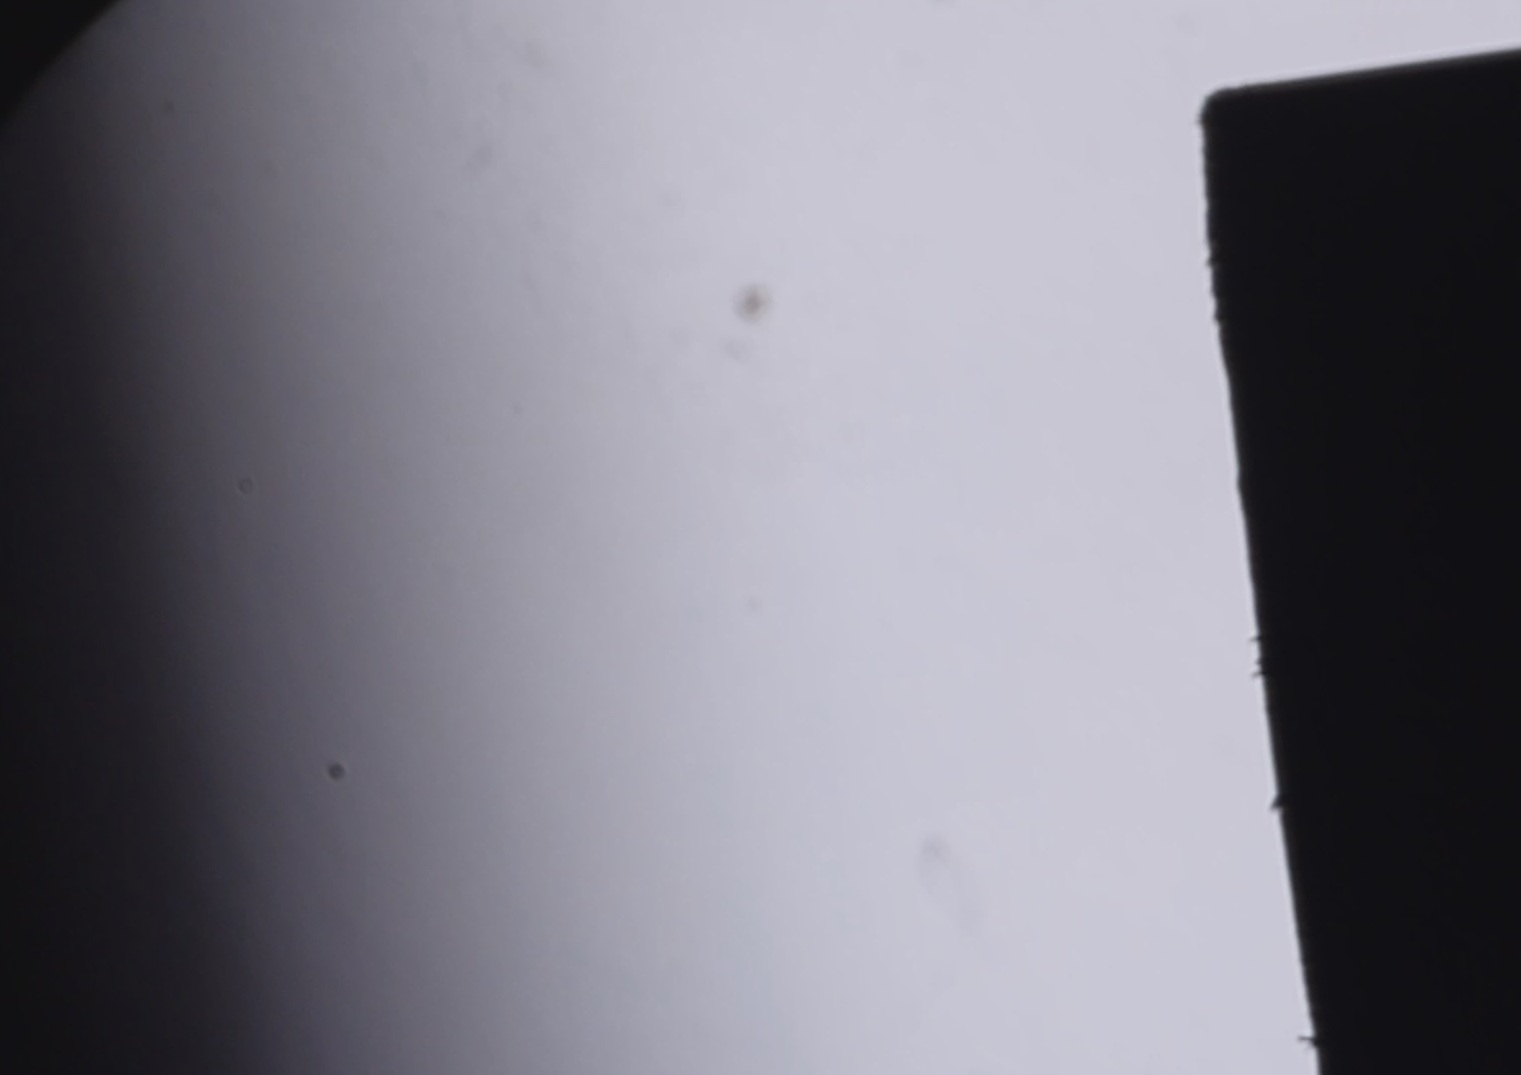
\includegraphics[scale = 0.12]{figures/choc_avant.jpg}
	\caption{\small{\textit{Image précédant l'onde de choc}}}
	\label{fig:choc_avant}
\end{figure}
\begin{figure}[H]
	\centering
	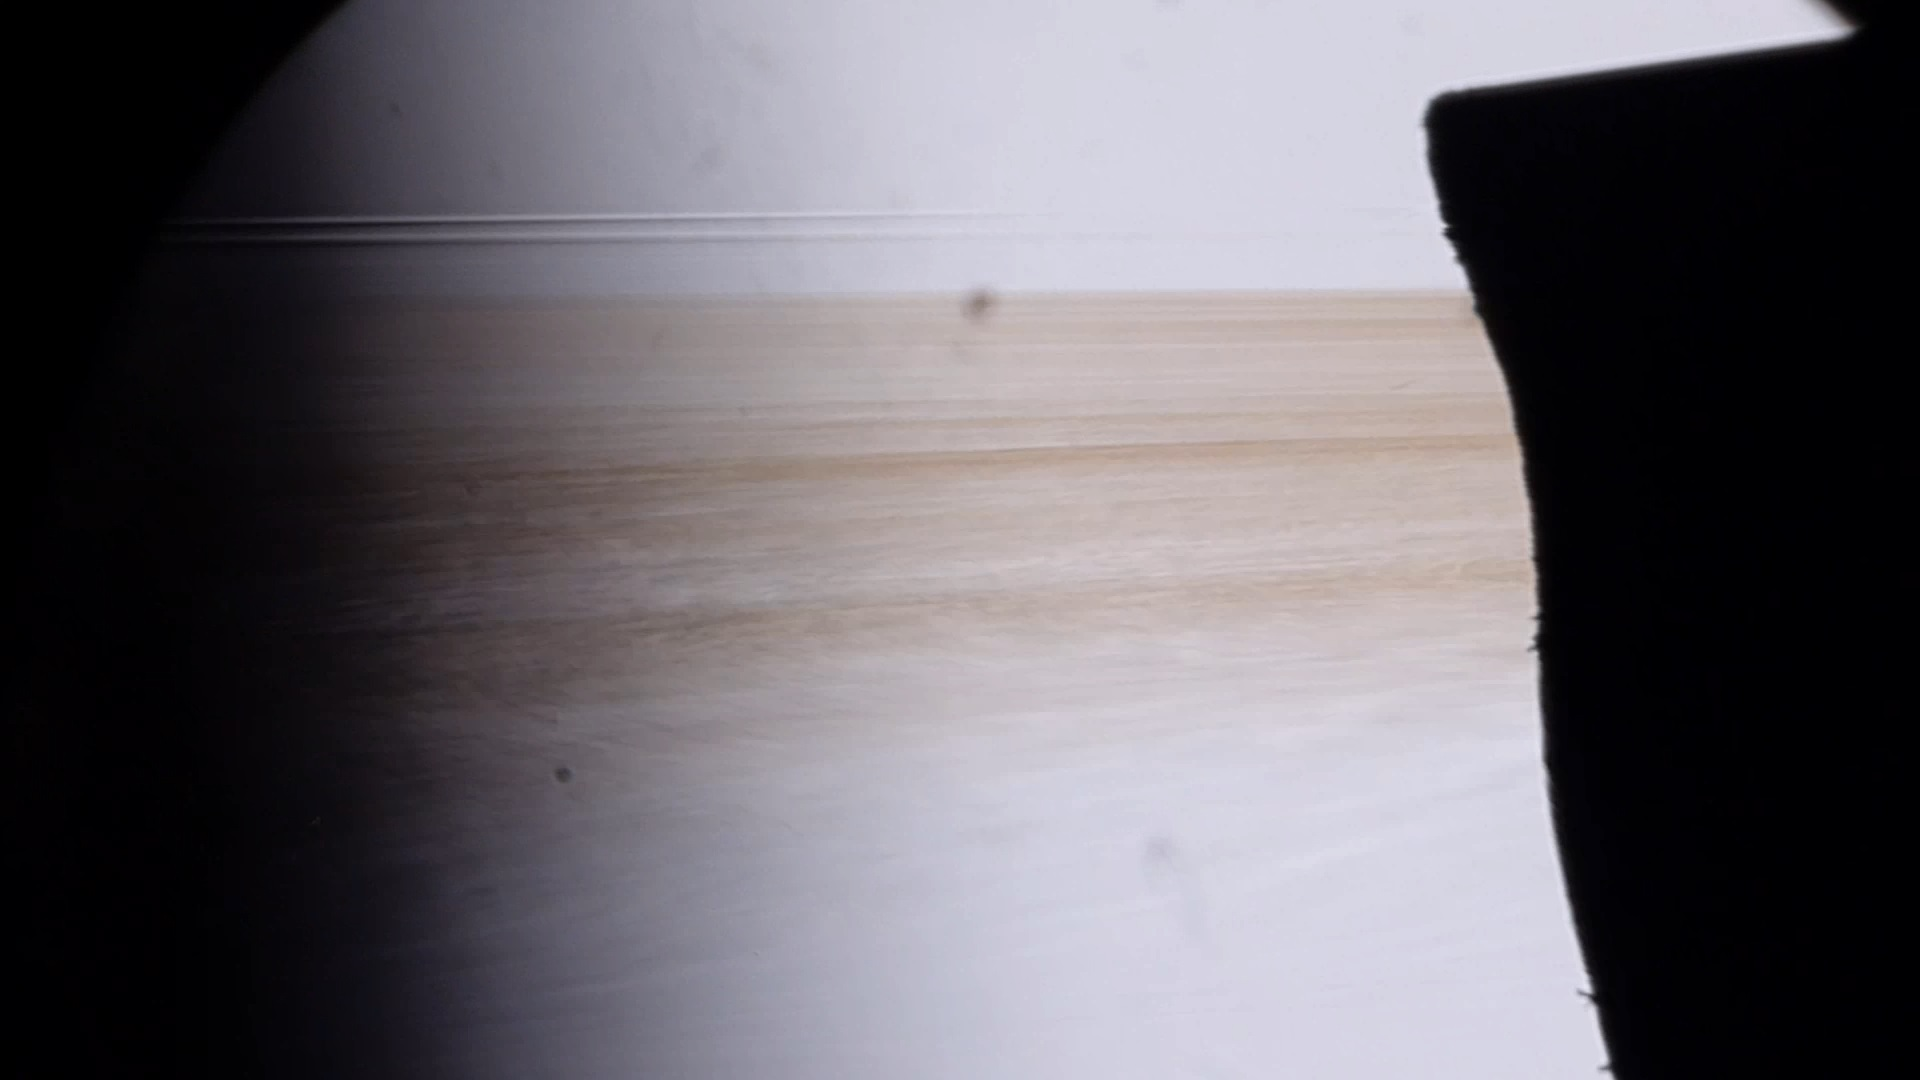
\includegraphics[scale = 0.12]{figures/choc_schlieren.jpg}
	\caption{\small{\textit{Cône de pression lié à l'onde choc, pression avant rupture : 2,5 bars}}}
	\label{fig:choc_schlieren}
\end{figure}
\begin{figure}[H]
	\centering
	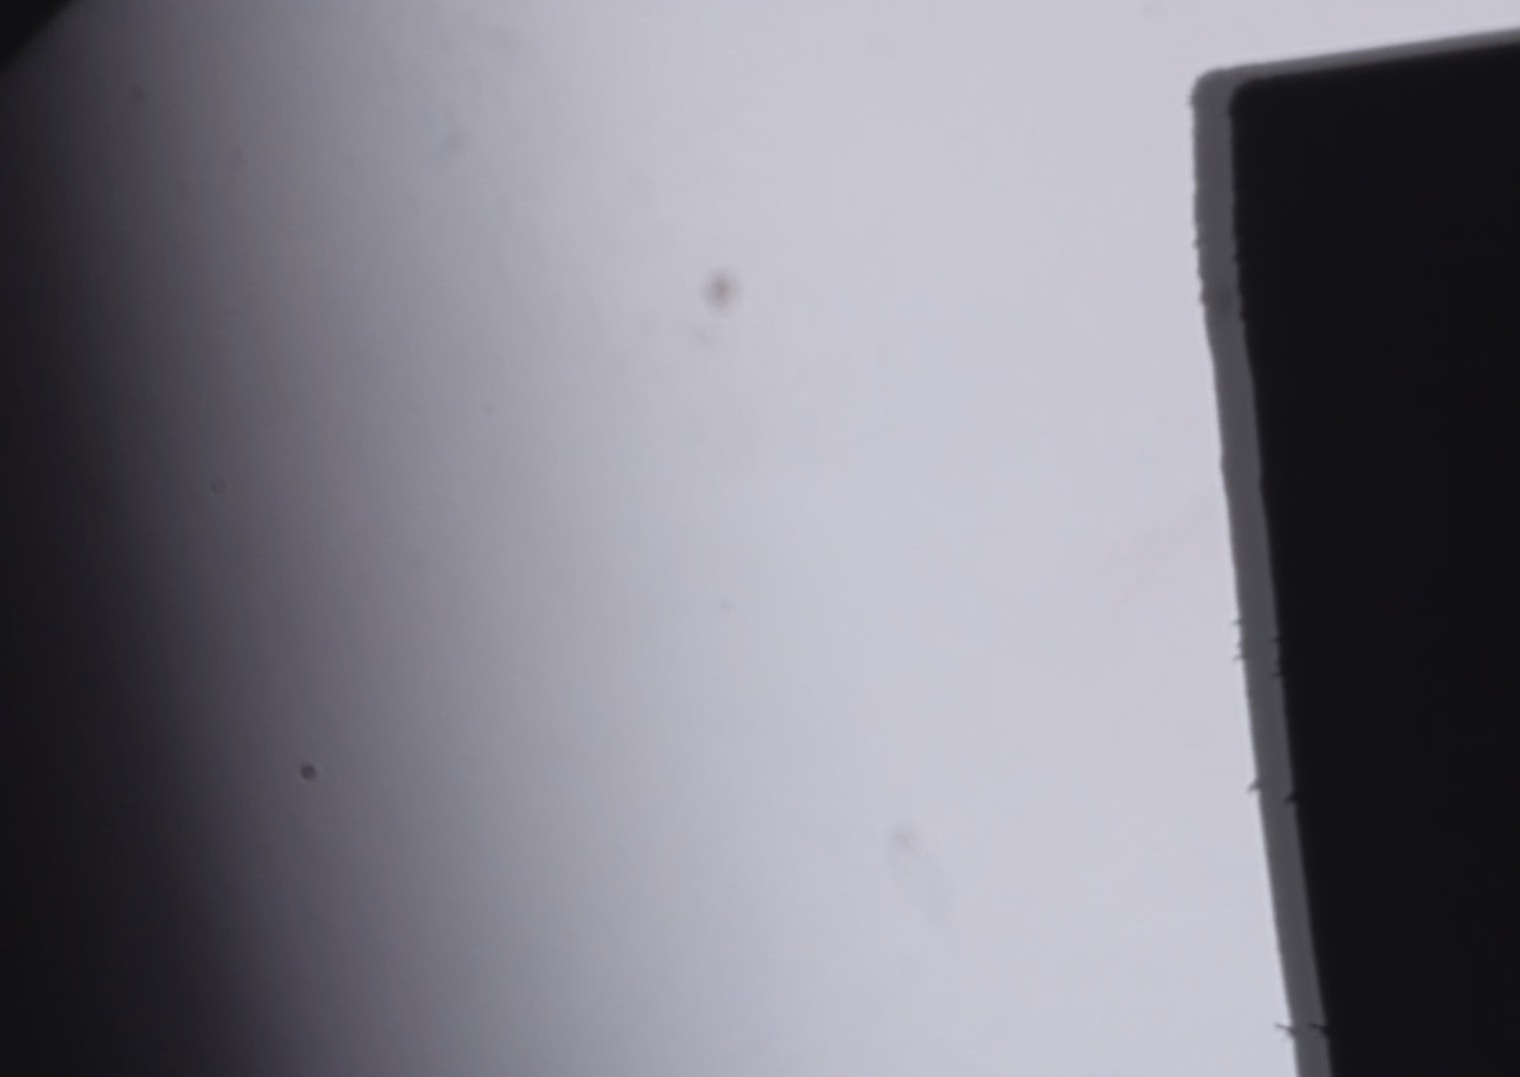
\includegraphics[scale = 0.12]{figures/choc_apres.jpg}
	\caption{\small{\textit{Image succédant l'onde de choc}}}
	\label{fig:choc_apres}
	\end{figure}
Faute de pouvoir observer le front d’onde par manque de moyens techniques on peut toutefois observer des “résidus” de l’onde de choc qui persistent plus longtemps sur la surface observable.\\\\
L’image~\ref{fig:choc_schlieren} n’est évidemment pas le front d’onde de l’onde de choc mais elle en est une conséquence directe: elle est unique donc de durée inférieure à $\frac{1}{60}$ = \textbf{17 ms} (les images la précédant (\ref{fig:choc_avant}) et la succédant (\ref{fig:choc_apres}) sont sans lien avec elle), et on observe clairement la projection de la fumée et la délimitation de pression horizontale qui en résulte.
De plus, on observe la déformation du tuyau sous l’effet de la libération de l’onde de choc.\\\\
Ces éléments permettent de conclure sur le fait que l’image observée est bien une conséquence du passage du front d’onde de l’onde de choc. Cependant, elle est difficilement observable même avec l'appareil photo disponible vu sa vitesse élevée.
